\section{RAS\_\-stack\_\-t::RAS\_\-stack\_\-t::RAS\_\-stack\_\-chkpt\_\-t Class Reference}
\label{classRAS__stack__t_1_1RAS__stack__chkpt__t}\index{RAS\_\-stack\_\-t::RAS\_\-stack\_\-chkpt\_\-t@{RAS\_\-stack\_\-t::RAS\_\-stack\_\-chkpt\_\-t}}
Inheritance diagram for RAS\_\-stack\_\-t::RAS\_\-stack\_\-t::RAS\_\-stack\_\-chkpt\_\-t:\nopagebreak
\begin{figure}[H]
\begin{center}
\leavevmode
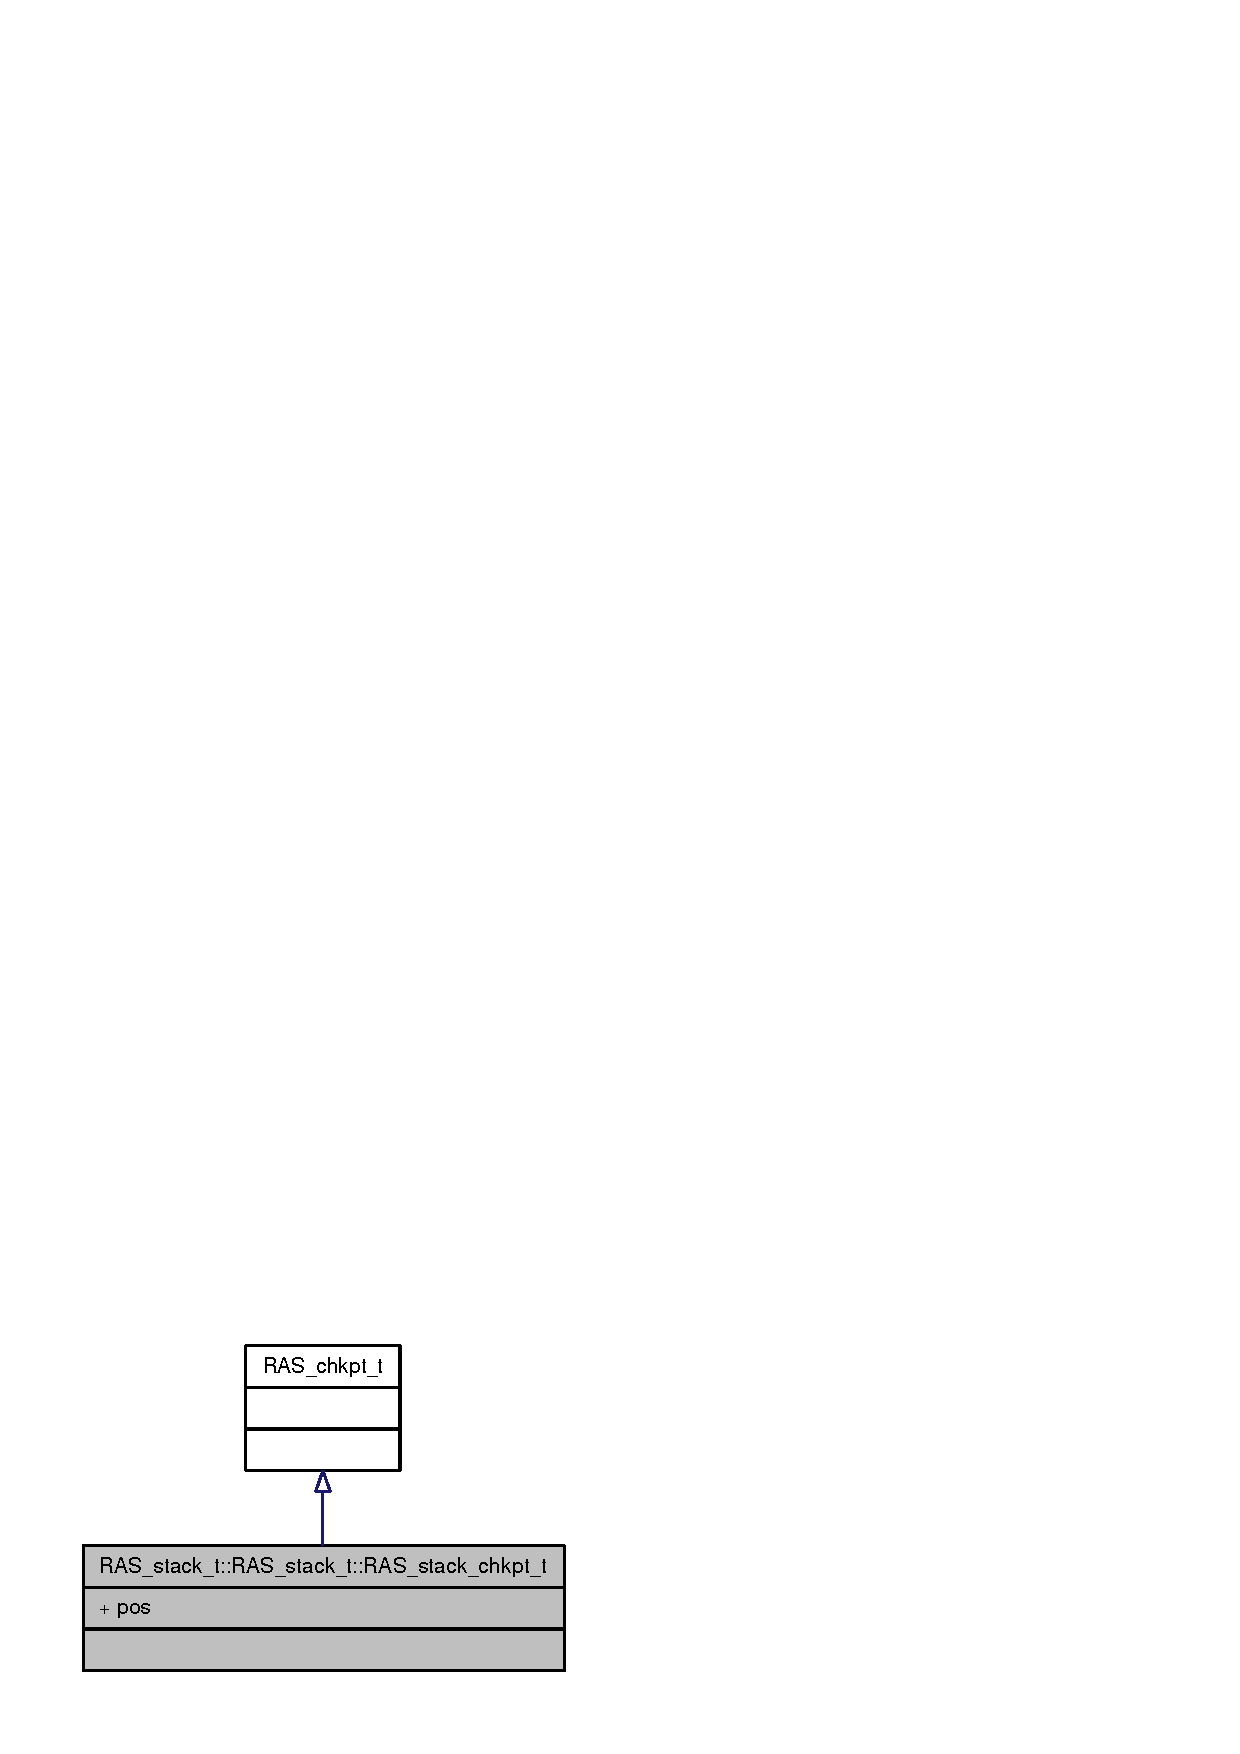
\includegraphics[width=274pt]{classRAS__stack__t_1_1RAS__stack__chkpt__t__inherit__graph}
\end{center}
\end{figure}
Collaboration diagram for RAS\_\-stack\_\-t::RAS\_\-stack\_\-t::RAS\_\-stack\_\-chkpt\_\-t:\nopagebreak
\begin{figure}[H]
\begin{center}
\leavevmode
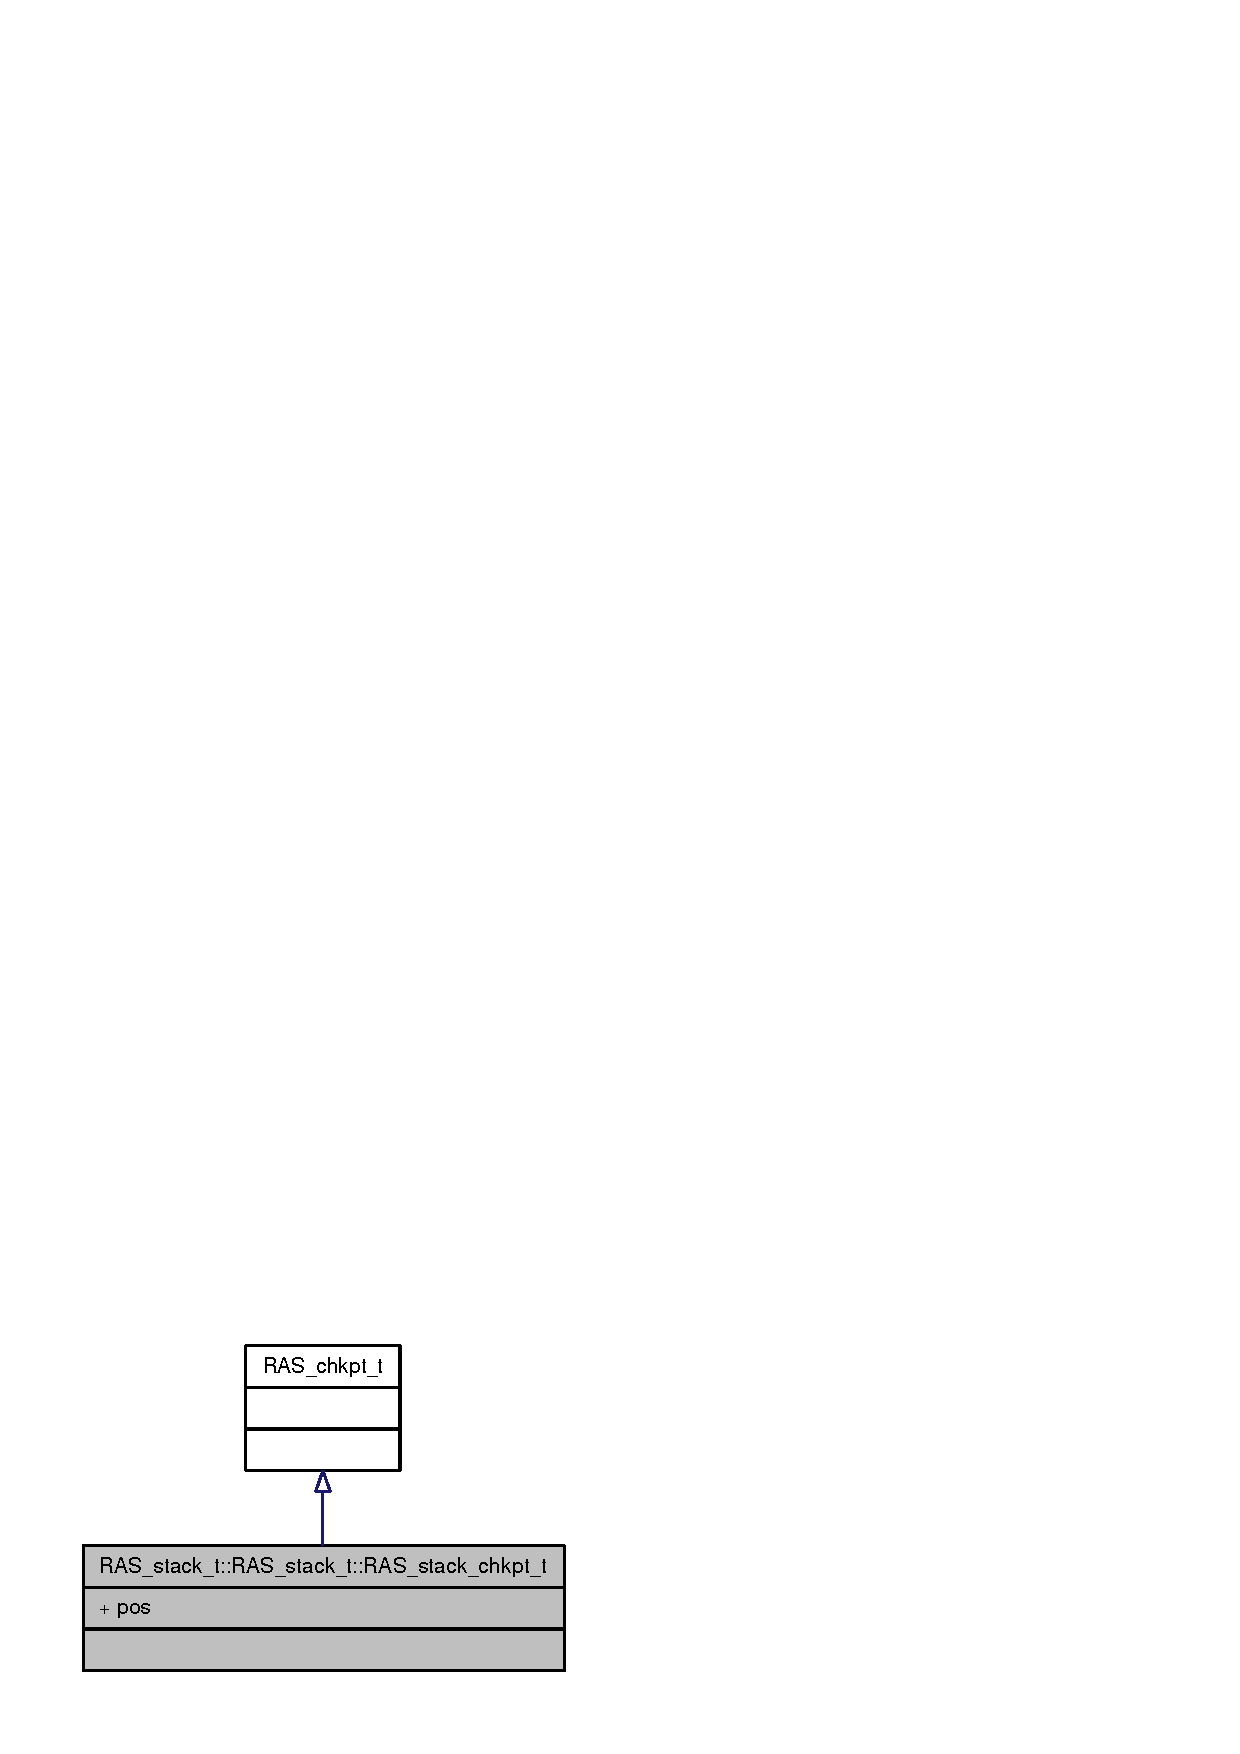
\includegraphics[width=274pt]{classRAS__stack__t_1_1RAS__stack__chkpt__t__coll__graph}
\end{center}
\end{figure}
\subsection*{Public Attributes}
\begin{CompactItemize}
\item 
int {\bf pos}
\end{CompactItemize}


\subsection{Detailed Description}


Definition at line 20 of file ras-stack.cpp.

\subsection{Member Data Documentation}
\index{RAS\_\-stack\_\-t::RAS\_\-stack\_\-chkpt\_\-t@{RAS\_\-stack\_\-t::RAS\_\-stack\_\-chkpt\_\-t}!pos@{pos}}
\index{pos@{pos}!RAS_stack_t::RAS_stack_chkpt_t@{RAS\_\-stack\_\-t::RAS\_\-stack\_\-chkpt\_\-t}}
\subsubsection[{pos}]{\setlength{\rightskip}{0pt plus 5cm}int RAS\_\-stack\_\-t::RAS\_\-stack\_\-t::RAS\_\-stack\_\-chkpt\_\-t::pos}\label{classRAS__stack__t_1_1RAS__stack__chkpt__t_7281fcb88520e943302cd6b777477fb2}




Definition at line 23 of file ras-stack.cpp.

The documentation for this class was generated from the following file:\begin{CompactItemize}
\item 
{\bf ras-stack.cpp}\end{CompactItemize}
